\documentclass{ctexart}
\usepackage{tikz}
\usepackage{indentfirst}
\usepackage{hyperref}
\usetikzlibrary{arrows, decorations.pathmorphing, backgrounds, positioning, fit, petri, automata}
\definecolor{yellow1}{rgb}{1,0.8,0.2}

\setlength{\parindent}{2cm}


\author{xzx}
\title{assignment3我的答案}


\begin{document}
\maketitle
\setcounter{page}{0}
\thispagestyle{empty}
\newpage

%\begin{flushleft}



\section{Q1: Image Captioning with Vanilla RNNs}


\subsection{Recurrent Neural Networks}
首先是单个神经元的前向与后向传播。一个神经元的示意图如图
\ref{fig:rnn_step_forward}所示.\\

\begin{figure}[h]


  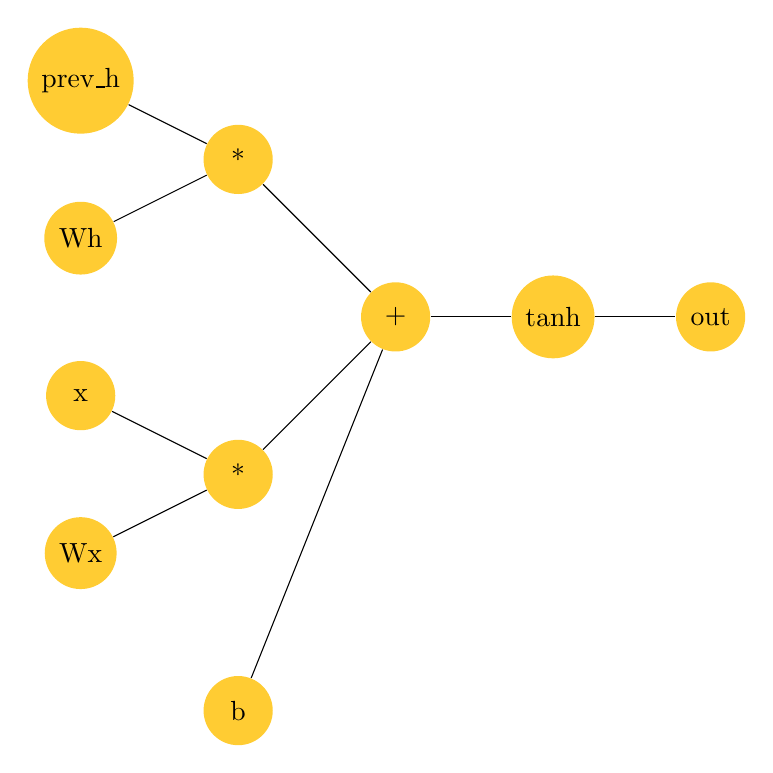
\begin{tikzpicture}
    \tikzstyle{every state} = [fill=yellow1,draw=none,text=black]
    \node[state] (p_h)             at (-4,8) {prev\_h};
    \node[state] (wh)              at (-4,6) {Wh};
    \node[state] (x)               at (-4,4) {x};
    \node[state] (Wx)              at (-4,2) {Wx};
    \node[state] (b)               at (-2,0) {b};
    \node[state] (mul1)            at (-2,7) {*};
    \node[state] (mul2)            at (-2,3) {*};
    \node[state] (add)             at (0,5)  {+};
    \node[state] (tanh)            at (2,5)  {tanh};
    \node[state] (out)             at (4,5)  {out};

    \path (p_h)     edge              node {}  (mul1)
          (wh)      edge              node {}  (mul1)
          (x)       edge              node {}  (mul2)
          (Wx)      edge              node {}  (mul2)
          (mul1)    edge              node {}  (add)
          (mul2)    edge              node {}  (add)
          (b)       edge              node {}  (add)
          (add)     edge              node {}  (tanh)
          (tanh)    edge              node {}  (out);

  \end{tikzpicture}
\caption{rnn\_step\_forward}
\label{fig:rnn_step_forward}
\end{figure}

反向传播也很容易根据这个图示推导出来.\\
\indent 整个rnn的前向与后向传播再课程里面已经把图给话出来了。这里面Wh 还有Wx被重复使用了很多遍。
对于一个变量后分成多条路径的,把这几条路径上面的微分相加。

\subsection{RNN for image captioning}
rnn的输入有点多,看上去有些混乱,整理一下输入放在图\ref{fig:rnn for image captioning}
中可以看的清楚一些。以图
\ref{fig:rnn_sample_input}为例作为输入.\\
\begin{figure}
  \includegraphics[width=5in]{./assignment1_pic/rnn_caption_sample.png}
  \caption{sample\_input}
  \label{fig:rnn_sample_input}
\end{figure}

\begin{figure}
  \includegraphics[width=5in]{./assignment1_pic/rnn_caption_train.jpg}
  \caption{RNN for image captioning}
  \label{fig:rnn for image captioning}
\end{figure}

每个神经元的输出会同时传给下个神经元并且向上传到上一层网络。这个ipynb的最开始就说已经帮我们
把图像的特征提取出来了,因此feature当做最初的h0传入网络就好了。每个单词对应的向量作为x从下面
输入到网络。


\section{Q2: Image Captioning with LSTMs}
人类在进行学习的时候,实际上会忘掉一些东西。比如一些东西很久没有通过了就会忘掉。LSTM就是
rnn在这个基础上面的变化。\\
\indent 课程的PPT里有几个从论文里面摘下来的图,我觉得这几个图不是很好理解,我在这几张图的基础上做一些
改变,结合作业中的代码希望能够更清楚的解释lstm。下面都默认忽略掉bias,这样画图能简单些。\\
\begin{figure}
  \includegraphics[width=5in]{./assignment1_pic/LSTM_cell.jpg}
  \caption{LSTM cell}
  \label{fig:LSTM cell}
\end{figure}
如图\ref{fig:LSTM cell},输入的x跟hidden layer跟原来差不多,输出从原来的H变成了现在的
4H。要把这个4H平均分成四份,每一份代表了一个门。i表示输入;f表示forget,就是前面说的要忘记
一些东西;o表示输出;g表示什么视频中说他也不知道,反正就是一个门。然后下一层的h要有这些一起
来决定。公式ppt里都有。\\
\indent 这样,标准的rnn的图就改成了ppt第68页的图,原来的hidden layer只有一个绿色的框,现在在
绿框下面增加了一个黄色的框,就是公式里面的c,表示cell。\\
\indent 把模型实现了以后可以看到它会学习看图说话。有些图片说出来的话挺搞笑的。




\section{Q3: Image Gradients: Saliency maps and Fooling Images }
这一节主要的想法是利用反向传播修改原图片,假如微小的噪声后使原图片被误分类。ImageGradients.ipynb
中数据加载要2.8GB的内存,所以建议如果电脑的内存只有4G的话,尽量先去把代码写好,然后再加载数据。
尽量加载一次数据多做一些事情。反正我每次都有大概十分钟浪费在加载数据上面。\\
\subsection{Saliency Maps}
题目中说要先去读一读参考文献的第二章,这篇论文百度就可以找到。
(这一块作业好像写的有点问题,容我再看看。。)

\subsection{Fooling Images}
这一小段的目的就是要把原来的图片做细小的更改,使得cnn会误分类。\\
\indent 首先把图片正常的前向传播,会得到一个当前图片的分类。因为用的都是筛选过的validation
的数据,所以第一次得到的分类肯定是正确的。假设正确的分类是a,目标是把产生一个相似的图片,使得
误分类为b。那么第一次前向传播得到的结果肯定是a,然后将a与b之间求损失函数的值,再反向传播回去。
模型中都会输出一个dx,把原来的图片减去dx就好。有可能一部分像素被减成负的了,在输出图片的时候
取绝对值输出。



%\end{flushleft}


\end{document}
